\section{Midlands Catchment Runoff  Model (model ID: 39)}
The Midlands Catchment Runoff model (fig.~\ref{fig:39_schematic}) is intended to be used in a flood-forecasting setting \citep{Moore2001}. To reduce the number of free parameters, the original evaporation routines and routing are somewhat simplified here. The model has 5 stores and 16 parameters ($S_{max}$, $c_{max}$, $c_0$, $c_1$, $c_e$, $D_{surp}$, $k_d$, $\gamma_d$, $q_{p,max}$, $k_g$, $\tau$, $S_{bf}$, $k_{cr}$, $\gamma_{cr}$, $k_{or}$ and $\gamma_{or}$). The model aims to represent:

\begin{itemizecompact}
\item Interception by vegetation;
\item Direct runoff from a variable contributing area;
\item A deficit-based approach to soil moisture accounting and interflow and percolation;
\item Baseflow from groundwater;
\item Uniform flood flood wave distribution in time;
\item In-channel and out-of-channel flood routing.
\end{itemizecompact}

\subsection{MARRMoT model name}
m\_39\_mcrm\_16p\_5s \\

% Equations
\subsection{Model equations}

% Model layout figure
{ 																	% This ensures it doesn't warp text further down
\begin{wrapfigure}{l}{5cm}
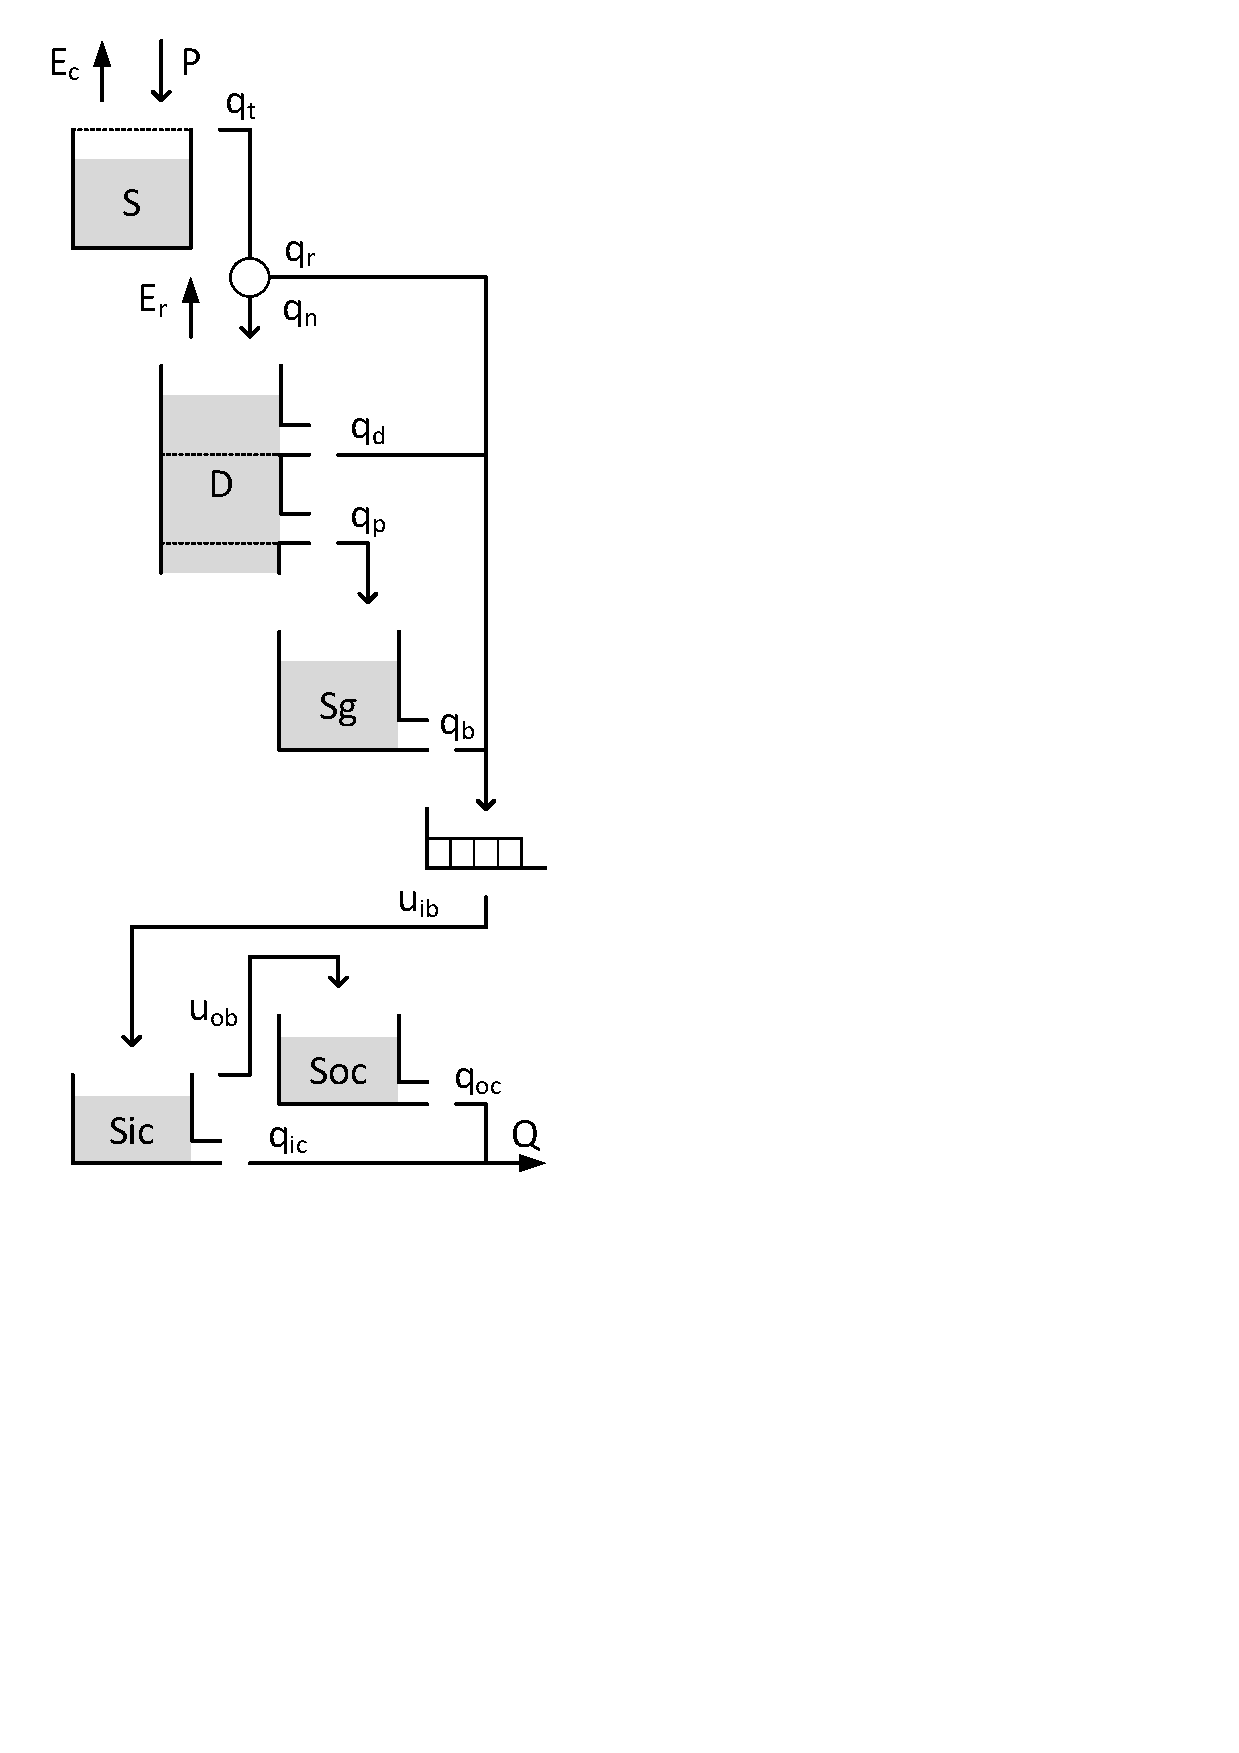
\includegraphics[trim=1cm 10cm 7cm 1cm,width=7cm,keepaspectratio]{./AppA_files/39_schematic.pdf}
\caption{Structure of the MCR model} \label{fig:39_schematic}
\end{wrapfigure}

\begin{align}
	\frac{dS}{dt} &= P-E_c-q_t \\
	E_c &= \begin{cases}
		E_p, &\text{if } S > 0 \\
		0, & \text{otherwise} \\
	\end{cases} \\
	q_t &= 
	\begin{cases}
		P, & \text{if } S=S_{max} \\
		0, & \text{otherwise}
	\end{cases}
\end{align}

Where $S$ [mm] is the current interception storage, refilled by precipitation $P$ $[mm/d]$ and drained by evaporation $E_c$ $[mm/d]$ and throughfall $q_t$ $[mm/d]$.
$E_c$ occurs at the potential rate whenever possible.
$q_t$ occurs only when the store is at maximum capacity $S_{max}$ [mm].

\begin{align}
	\frac{dD}{dt} &= q_n - E_r -q_d-q_p\\
	q_n &=q_t-q_r\\
	q_r &= min\left(c_{max},c_0+c_0e^{c_1D}\right)*q_t\\
	E_r &= \frac{1}{1+e^{-c_eD}}*\left(E_p-E_c\right)\\
	q_d&= \begin{cases}
		k_d\left(D_{surp}-D\right)^{\gamma_d}, &\text{if } D > D_{surp} \\
		0, &\text{otherwise} \\
	\end{cases} \\
	q_p &= \begin{cases}
		q_{p,max}, & \text{if } D\geq D_{surp} \\
		\frac{D}{D_{surp}}q_{p,max}, & \text{if } 0 < D < D_{surp}\\
		0, & \text{otherwise}
	\end{cases}
\end{align}
} % end of wrapfigure fix

Where $D$ [mm] is the current storage in soil moisture, refilled by net infiltration $q_n$ $[mm/d]$ and drained by evaporation $E_r$ $[mm/d]$, direct runoff $q_d$ $[mm/d]$ and percolation $q_p$ $[mm/d]$. 
Negative D-values are possible and indicate a moisture deficit. 
Net inflow $q_n$ is calculated as the difference between throughfall $q_t$ and rapid runoff $q_r$ $[mm/d]$.
$q_r$ varies depending on the current degree of saturation in the catchment, with a maximum fraction of the catchment area contributing to rapid runoff called $c_{max}$ [-], a minimum contributing area of $c_0$ [-] and an exponential increase with increasing soil moisture storage, controlled through shape parameter $c_1$ [-], in between.
$E_r$ fulfils any remaining evaporation demand but decreases with increasing moisture deficit (negative D values).
This relation is controlled through shape parameter $c_2$.
$q_d$ has a non-linear relation with storage above a threshold $D_{surp}$ [mm] through time scale parameter $k_d$ $[d^{-1}]$ and non-linearity parameter $\gamma_d$ [-].
Percolation $q_p$ has a maximum rate of $q_{p,max}$ if D is above threshold $D_{surp}$ and decreases linearly between $D=D_{surp}$ and $D=0$.

\begin{align}	
	\frac{dS_g}{dt} &= q_p - q_b\\
	q_b &= k_g*S_g^{1.5}
\end{align}
  
Where $S_g$ [mm] is the current groundwater storage, refilled by percolation $q_p$ and drained by baseflow $q_b$ $[mm/d]$.
$q_b$ uses time parameter $k_g$ $[d^{-1}]$ and a fixed non-linearity coefficient of 1.5. 
Next, $q_r$, $q_d$ and $q_b$ are summed together and distributed uniformly over timespan $\tau$ [d], giving delayed flow $u_{ib}$ $[mm/d]$.

\begin{align}
	\frac{dS_{ic}}{dt} &= u_{ib} - u_{ob} - q_{ic}\\
	u_{ob} &= \begin{cases}
		u_{ib}, & \text{if } S_{ic}=S_{bf} \\
		0, & \text{otherwise}\\
	\end{cases}\\
	q_{ic} &= \begin{cases}
		k_{cr}*S_{ic}^{\gamma_{cr}}, & \text{if } q_{ic}<\frac{3}{4}S_{ic} \\
		\frac{3}{4}S_{ic}, & \text{otherwise}
	\end{cases}
\end{align}

Where $S_{ic}$ [mm] is the current in-channel storage, refilled by $u_{ic}$ and drained by in-channel flow $q_{ic}$  $[mm/d]$ and out-of-bank flow $u_{ob}$  $[mm/d]$.
$u_{ob}$ only occurs when the store is at maximum capacity $S_{bf}$ [mm].
$q_{ic}$ uses time parameter $k_{cr}$ $[d^{-1}]$ and non-linearity parameter $\gamma_{cr}$ [-].

\begin{align}
	\frac{dS_{oc}}{dt} &= u_{ob} - q_{oc} \\
	q_{oc} &= \begin{cases}
		k_{or}*S_{oc}^{\gamma_{or}}, & \text{if } q_{oc}<\frac{3}{4}S_{oc} \\
		\frac{3}{4}S_{oc}, & \text{otherwise}
	\end{cases} 
\end{align}

Where $S_{oc}$ [mm] is the current out-of-channel storage, refilled by $u_{ob}$ and drained by out-of-channel flow $q_{oc}$  $[mm/d]$.
$q_{oc}$  uses time parameter $k_{or}$ $[d^{-1}]$ and non-linearity parameter $\gamma_{or}$ [-]. Total flow:

\begin{align}
	Q_t &= q_{oc}+q_{ic}
\end{align}

\newpage
\subsection{Parameter overview}
% Table generated by Excel2LaTeX from sheet 'Sheet1'
\begin{table}[htbp]
  \centering
    \begin{tabular}{lll}
    \toprule
    Parameter & Unit  & Description \\
    \midrule
    $S_{max}$ & $mm$  & Maximum interception storage \\
    $c_{max}$ & $-$   & Maximum fraction of area contributing to rapid runoff \\
    $c_0$ & $-$   & Minimum fraction of area contributing to rapid runoff \\
    $c_1$ & $-$   & Contributing area exponential shape parameter \\
    $c_e$ & $-$   & Evaporation exponential shape parameter \\
    $D_{surp}$ & $mm$  & Threshold for direct runoff generation \\
    $k_d$ & $d^{-1}$ & Runoff coefficient \\
    $\gamma_d$ & $-$   & Runoff non-linearity \\
    $q_{p,max}$ & $mm~d^{-1}$ & Maximum percolation rate \\
    $k_g$ & $d^{-1}$ & Runoff coefficient \\
    $\tau$ & $d$   & Unit Hydrograph time base \\
    $S_{bf}$ & $mm$  & Maximum groundwater storage \\
    $k_{cr}$ & $d^{-1}$ & Runoff coefficient \\
    $\gamma_{cr}$ & $-$   & Runoff non-linearity \\
    $k_{or}$ & $d^{-1}$ & Runoff coefficient \\
    $\gamma_{or}$ & $-$   & Runoff non-linearity \\
    \bottomrule
    \end{tabular}%
  \label{tab:addlabel}%
\end{table}%
